\documentclass[10pt,a4paper]{article}

\usepackage[utf8]{inputenc}
\usepackage[T1]{fontenc}
\usepackage[french]{babel}
\usepackage{amsmath,amssymb}
\usepackage{graphicx}
\usepackage{geometry}
\usepackage{multicol}
\usepackage{siunitx}
\usepackage{titlesec}

% --- Cadres ---
\usepackage[most]{tcolorbox}

\geometry{margin=1.4cm}
\setlength{\parindent}{0pt}
\setlength{\parskip}{2pt}
\pagenumbering{gobble}

% Alignement à gauche
\raggedright
\sloppy

% Environnement "section encadrée"
\newtcolorbox{metbox}[1]{%
  colback=white,
  colframe=black,
  boxrule=0.4pt,
  arc=0pt,                 % angles carrés
  left=2mm,right=2mm,top=1.2mm,bottom=1.2mm,
  boxsep=0mm,
  before skip=2mm,
  after skip=2mm,
  title=\textbf{#1}
}

\begin{document}

\begin{center}
{\Large \textbf{Mecatro 1 : Formulaire complet}}\\
{V0.0}
\end{center}

\begin{center}
{\Large \textbf{Circuits magnétiques}}
\end{center}

\begin{multicols}{2}

%====================================================
\begin{metbox}{Grandeurs}

\textbf{Électromagnétisme}

$\vec E$ : champ électrique [V/m] \\
$\vec D$ : déplacement électrique [C/m$^2$] \\
$\rho$ : densité volumique de charge [C/m$^3$] \\
$\vec J$ : densité de courant [A/m$^2$] \\
$i$ : courant électrique [A] \\
$u$ : tension [V] \\
$R$ : résistance électrique [$\Omega$] \\
$P$ : puissance électrique [W]

\medskip
\textbf{Magnétisme}

$\vec H$ : champ magnétique [A/m] \\
$\vec B$ : induction magnétique [T] \\
$\Phi$ : flux magnétique [Wb] \\
$\Psi$ : flux totalisé [Wb] \\
$\theta$ : force magnétomotrice (f.m.m.) [A.tours] \\
$R_m$ : réluctance magnétique [H$^{-1}$] \\
$\Lambda$ : perméance [H] \\
$L$ : inductance propre [H] \\
$L_{12}$ : inductance mutuelle [H] \\
$k$ : coefficient de couplage [-] \\
$\sigma$ : coefficient de dispersion [-]

\medskip
\textbf{Géométrie / matériaux}

$l$ : longueur du circuit magnétique [m] \\
$S$ : section [m$^2$] \\
$x$ : entrefer [m] \\
$n$ : nombre de spires [-] \\
$\mu$ : perméabilité [H/m] \\
$\mu_0$ : perméabilité du vide [H/m] \\
$\mu_r$ : perméabilité relative [-] \\
$\varepsilon$ : permittivité [F/m] \\
$\varepsilon_0$ : permittivité du vide [F/m] \\
$\rho$ : résistivité électrique [$\Omega\cdot$m]

\medskip
\textbf{Grandeurs dynamiques}

$v$ : vitesse [m/s] \\
$\alpha$ : angle mécanique [rad] \\
$\Omega$ : vitesse angulaire [rad/s] \\
$\omega$ : pulsation électrique [rad/s] \\
$f$ : fréquence [Hz] \\
$\delta$ : profondeur de peau [m] \\
$W$ : énergie magnétique [J] \\
$F$ : force de Laplace [N]

\end{metbox}

%====================================================
\begin{metbox}{Hypothèses pour l'analyse des circuits magnétiques}

Lors de l'analyse d'un circuit magnétique, on adopte généralement
les hypothèses simplificatrices suivantes :

\medskip
\textbf{Longueur moyenne du parcours}

Le champ magnétique est supposé uniforme dans le matériau et
le parcours du flux est modélisé par une \textbf{longueur moyenne}
$l$ du circuit magnétique.

\[
H \approx \frac{\theta}{l}
\]

\medskip
\textbf{Section constante}

La section du circuit est supposée constante :

\[
B=\frac{\Phi}{S}
\]

\medskip
\textbf{Absence de flux de fuite}

Tout le flux circule dans le circuit magnétique :

\[
\Phi_{total} \approx \Phi_{utile}
\]

On néglige donc les \textbf{flux de fuite}.

\medskip
\textbf{Pas d'effet de frange dans l'entrefer}

Dans l'entrefer, les lignes de champ sont supposées
rectilignes et confinées dans la section :

\[
S_{eff} \approx S
\]

\medskip
\textbf{Perméabilité du noyau}

Deux approximations sont souvent utilisées :

\[
\mu_r \gg 1
\quad \Rightarrow \quad
R_{m,fer} \approx 0
\]

ou bien

\[
\mu_r = \text{constante}
\]

ce qui permet d'utiliser la relation linéaire

\[
B=\mu H
\]

\end{metbox}

%====================================================
\begin{metbox}{Relations matériau}

\[
\vec B=\mu \vec H
\qquad
\mu=\mu_0\mu_r
\qquad
\mu_0=4\pi\cdot10^{-7}
\]

\[
\vec D=\varepsilon \vec E
\qquad
\varepsilon=\varepsilon_0\varepsilon_r
\]

\[
c_0=\frac{1}{\sqrt{\mu_0\varepsilon_0}}
\]

\end{metbox}

%====================================================
\begin{metbox}{Résistance, résistivité et température}

\[
\boxed{R=\rho\frac{l}{S}}
\qquad
\left[\rho\right]=\Omega\cdot\text{m}
\]

\[
G=\frac{1}{R}
\]

\[
\boxed{\rho = R\frac{S}{l}}
\]

\[
\boxed{\rho(T)=\rho(T_0)\left[1+\alpha\,(T-T_0)\right]}
\]

avec :
\[
\alpha : \text{coefficient de température } \left[\text{K}^{-1}\right],
\quad T \text{ en } ^\circ\text{C ou K}
\]

\end{metbox}

%====================================================
\begin{metbox}{Équations de Maxwell (quasi-statique)}

\[
\nabla\times \vec E=-\frac{\partial \vec B}{\partial t}
\]

\[
\nabla\times \vec H=\vec J
\]

\[
\nabla\cdot \vec B=0
\qquad
\nabla\cdot \vec D=\rho
\]

\end{metbox}

%====================================================
\begin{metbox}{Flux et potentiel magnétique}

\[
\Phi=\iint_S \vec B\cdot d\vec S
\]

\[
\theta=\oint_C \vec H\cdot d\vec l
\]

Si bobine $n$ spires :

\[
\theta = n i
\]

\end{metbox}


%====================================================
\begin{metbox}{Lois des circuits magnétiques}

\subsection*{Conservation du flux}

\[
\sum_i \Phi_i = 0
\]

Si flux constant :

\[
\Phi=B_1S_1=B_2S_2
\quad\Rightarrow\quad
B_2=B_1\frac{S_1}{S_2}
\]

\subsection*{Hopkinson (analogue Ohm)}

\[
\boxed{\theta = R_m \Phi}
\qquad
\boxed{\Phi=\Lambda \theta}
\]

\[
R_m=\frac{l}{\mu S}
\qquad
\Lambda=\frac{\mu S}{l}
\]

Série :
\[
R_{m,eq}=\sum R_m
\]

Parallèle :
\[
\frac{1}{R_{m,eq}}=\sum\frac{1}{R_m}
\]

\medskip
\textbf{Analogie électrique}

\[
u = R i
\qquad
R = \rho \frac{l}{S}
\qquad
P = U I
\]


\end{metbox}

%====================================================
\begin{metbox}{Entrefer}

\[
R_{m,fer}=\frac{l_{fer}}{\mu_0\mu_r S}
\]

\[
R_{m,x}=\frac{x}{\mu_0 S}
\]

\[
R_{eq}=R_{fer}+R_x
\]

\[
\Phi=\frac{n i}{R_{eq}}
\qquad
B=\frac{\Phi}{S}
\]

\[
\theta = H_{fer}l_{fer} + H_x x
\qquad
H_x=\frac{B}{\mu_0}
\]


Si $\mu_r\gg1$ :

\[
\boxed{B \approx \frac{\mu_0 n i}{x}}
\]

\begin{center}
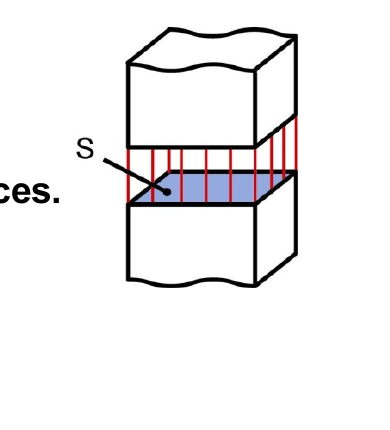
\includegraphics[width=0.40\linewidth]{assets/figures/p2-entrefer.png}
\end{center}

\end{metbox}

%====================================================
\begin{metbox}{Faraday}

Flux totalisé :

\[
\Psi=n\Phi
\]

\[
u_i=\pm\frac{d\Psi}{dt}
\]

Bobine résistive :

\[
u=Ri+\frac{d\Psi}{dt}
\]

\begin{center}
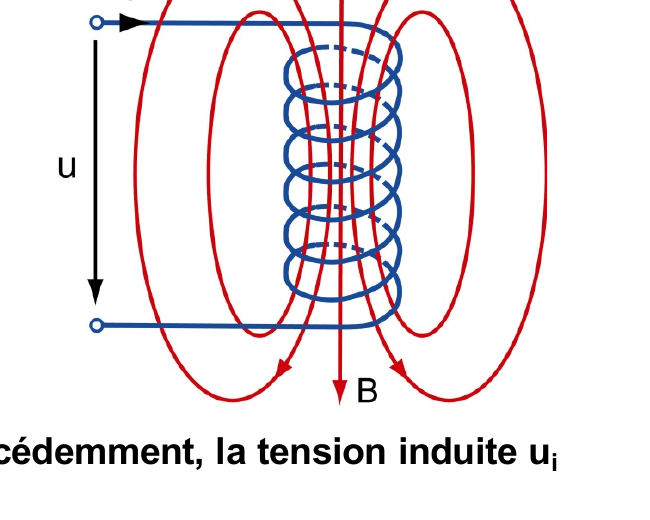
\includegraphics[width=0.54\linewidth]{assets/figures/p2-faraday.png}
\end{center}

\end{metbox}

%====================================================

\begin{metbox}{Inductance propre}

\[
\Psi=L i
\qquad
L=\frac{\Psi}{i}
\]

\[
L=n^2\Lambda
\]

\[
u_i=L\frac{di}{dt}
\]

Énergie :

\[
\boxed{W=\frac12 L i^2}
\]

\end{metbox}

%====================================================
\begin{metbox}{Inductance variable}

\[
u=L\frac{di}{dt}+i\frac{dL}{dt}
\]

Si $L=L(\alpha)$ :

\[
u=L\frac{di}{dt}+i\Omega\frac{dL}{d\alpha}
\]

\end{metbox}

%====================================================
\begin{metbox}{Inductances mutuelles}

\[
\Psi_1=L_{11}i_1+L_{12}i_2
\]

\[
\Psi_2=L_{22}i_2+L_{21}i_1
\]

\medskip
\textbf{Tensions induites}

\[
u_1 = R_1 i_1 + \frac{d\Psi_1}{dt}
\qquad
u_2 = R_2 i_2 + \frac{d\Psi_2}{dt}
\]

\[
u_1 = R_1 i_1 + L_{11}\frac{di_1}{dt}
      + L_{12}\frac{di_2}{dt}
\]

\[
u_2 = R_2 i_2 + L_{22}\frac{di_2}{dt}
      + L_{21}\frac{di_1}{dt}
\]

\[
L_{12} : \text{flux dans la bobine 1 créé par } i_2
\]

\[
L_{21} : \text{flux dans la bobine 2 créé par } i_1
\]

\[
L_{12}=L_{21}
\]

\[
L_{12}\le\sqrt{L_{11}L_{22}}
\]

\[
k=\frac{L_{12}}{\sqrt{L_{11}L_{22}}}
\qquad
\sigma=1-k^2
\]

\begin{center}
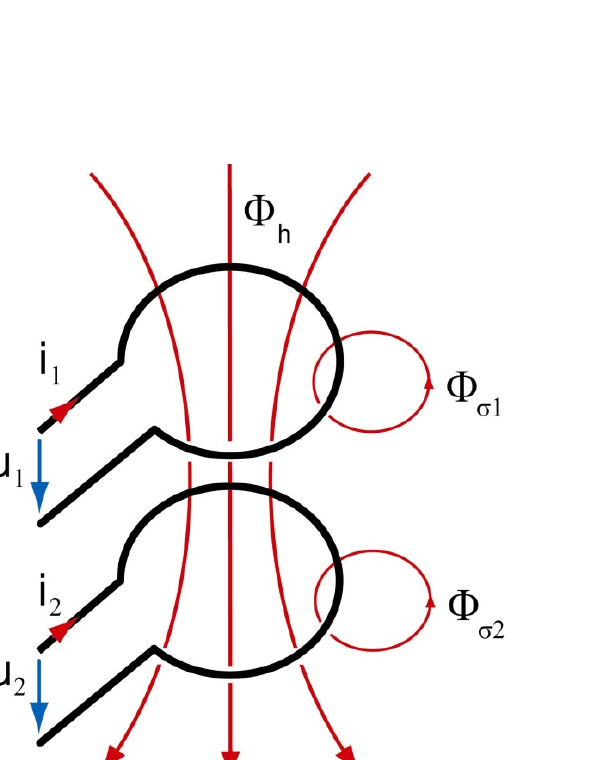
\includegraphics[width=0.62\linewidth]{assets/figures/p2-mutuelle.png}
\end{center}

\end{metbox}

%====================================================
\begin{metbox}{Loi Blv (tension de mouvement)}

\[
u=B l v
\]

Cas général :

\[
u=B l v \sin\alpha \cos\beta
\]

\begin{center}
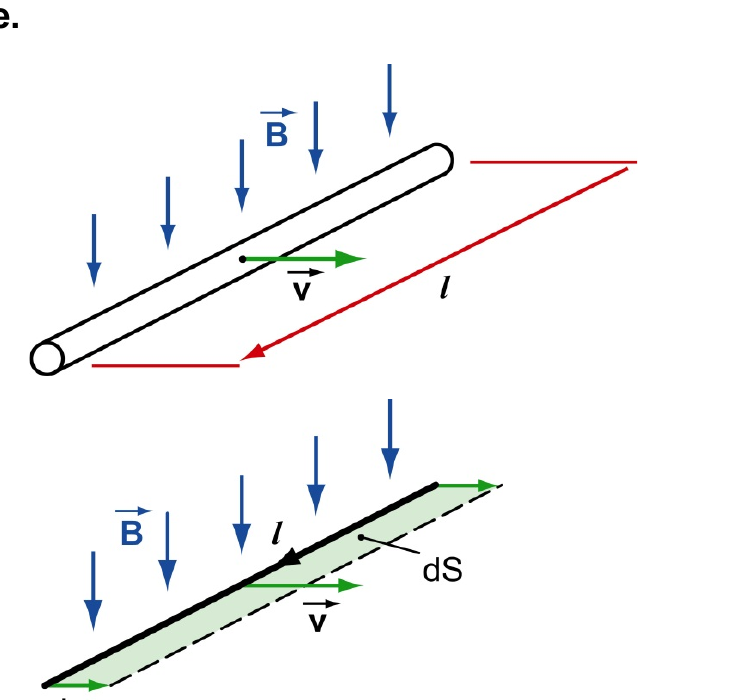
\includegraphics[width=0.62\linewidth]{assets/figures/p2-blv.png}
\end{center}

\end{metbox}

%====================================================
\begin{metbox}{Loi Bli (force de Laplace)}

\[
\vec F=i \vec l \times \vec B
\]

\[
F=B l i \sin\alpha
\]

$n$ conducteurs :

\[
F=n B l i
\]

\begin{center}
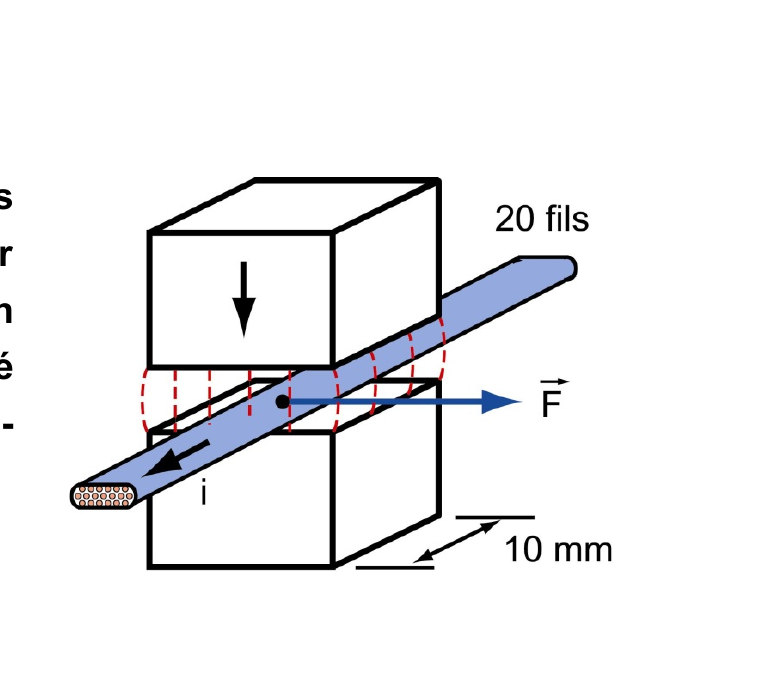
\includegraphics[width=0.62\linewidth]{assets/figures/p2-bli.png}
\end{center}

\end{metbox}

%====================================================
\begin{metbox}{Effet pelliculaire}

\[
\delta=\sqrt{\frac{2\rho}{\omega\mu}}
\qquad
\omega=2\pi f
\]

\end{metbox}

\end{multicols}

\newpage
\begin{center}
{\Large \textbf{Matériaux}}
\end{center}

\begin{multicols}{2}

%====================================================
\begin{metbox}{Magnétisation de la matière}

\[
\vec B=\mu_0(\vec H+\vec M)
\qquad
\vec B=\mu_0\vec H+\vec J
\]

\[
\vec J=\mu_0\vec M
\]

\[
\vec M=\chi\vec H
\]

\[
\vec B=\mu_0(\chi+1)\vec H
\qquad
\mu_r=\chi+1
\]

\[
\mu=\frac{dB}{dH}
\]

\begin{center}
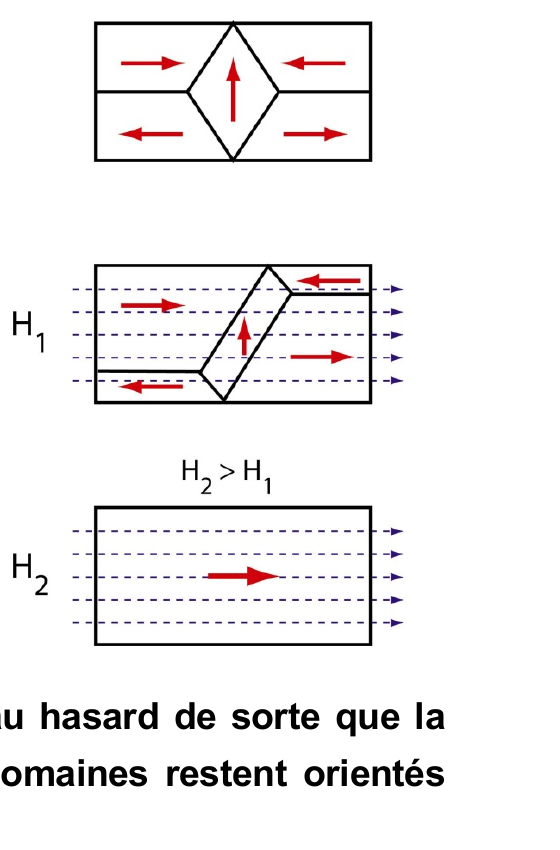
\includegraphics[width=0.56\linewidth]{assets/figures/p3-domaines.png}
\end{center}

\end{metbox}

%====================================================
\begin{metbox}{Moment magnétique}

\[
\vec m=i\vec A
\]

\end{metbox}

%====================================================
\begin{metbox}{Aimants permanents}

\[
B=\mu_0\mu_{ra}H+B_r
\]

\[
\mu_{ra}\approx 1.04 \text{ à } 1.4
\]

\[
B_r(T)=B_{r,20^\circ\mathrm{C}}
\left[1+K_{Br}(T-20)\right]
\]

\[
K_{Br}<0
\]

\[
(BH)_{\max}=\max\left(|B\cdot H|\right)
\]

\begin{center}
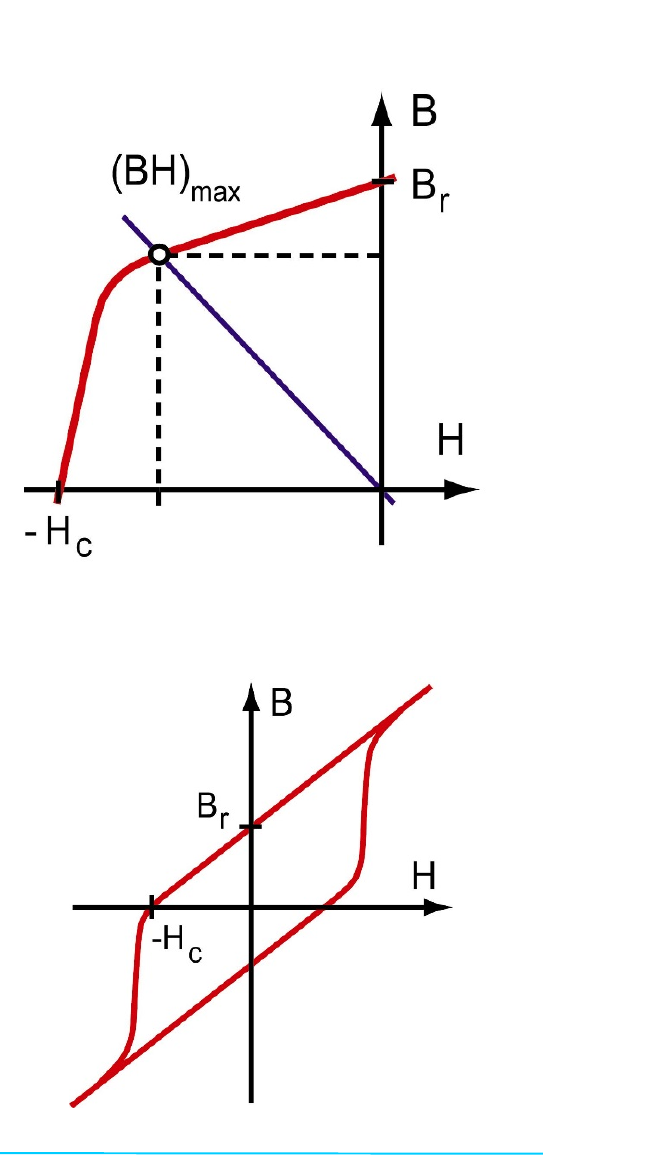
\includegraphics[width=0.60\linewidth]{assets/figures/p3-aimant-bh.png}
\end{center}

\end{metbox}

%====================================================
\begin{metbox}{Droite de charge (aimant + entrefer)}

\[
H_a l_a + H_e l_e = 0
\]

\[
B_a S_a=B_e S_e
\]

\[
B_e=\mu_0 H_e
\]

\[
\boxed{
B_a=-\mu_0\frac{S_e}{S_a}\frac{l_a}{l_e}H_a
}
\]

\begin{center}
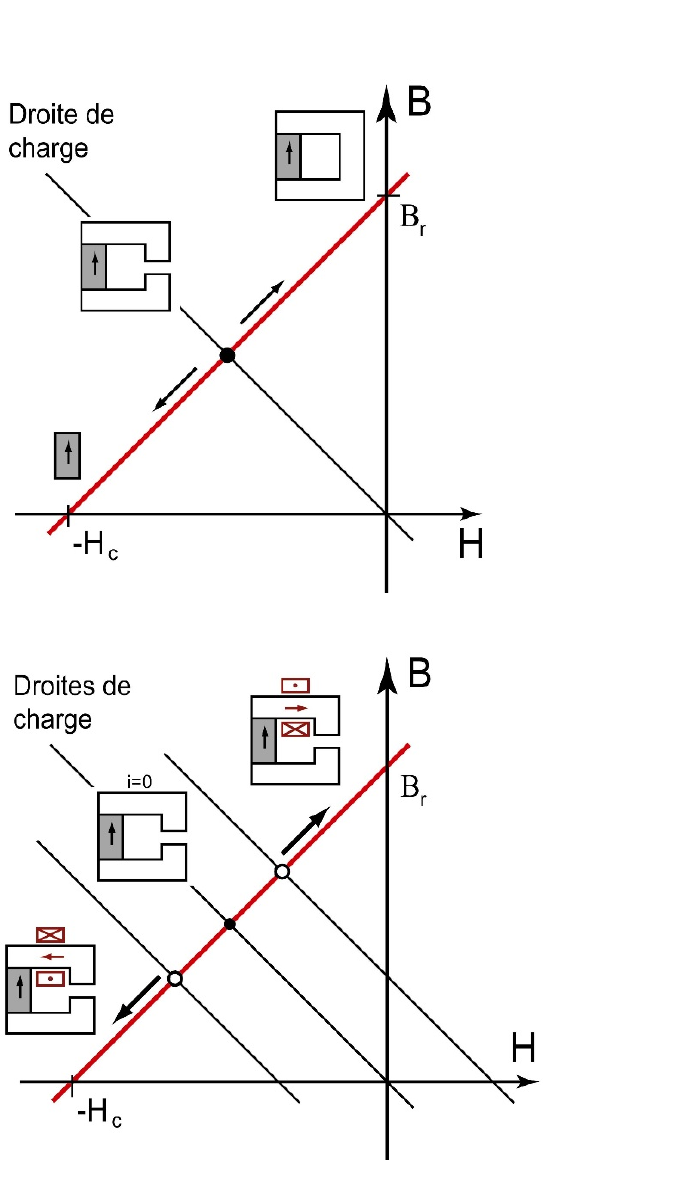
\includegraphics[width=0.60\linewidth]{assets/figures/p3-droite-charge.png}
\end{center}

\end{metbox}

\end{multicols}

\begin{center}
{\Large \textbf{Conversion électromécanique}}
\end{center}

{\small
\begin{multicols}{2}

%====================================================
\begin{metbox}{Bilan énergétique}

\[
dW_{el}=dW_{mec}+dW_{th}+dW_{mag}
\]

Pour un enroulement :
\[
u=Ri+\frac{d\Psi}{dt}
\]

Avec un degré de liberté linéaire $x$ :
\[
dW_{mag}=i\,d\Psi-F_x\,dx
\]

Cas rotatif :
\[
dW_{mag}=i\,d\Psi-T\,d\alpha
\]

\begin{center}
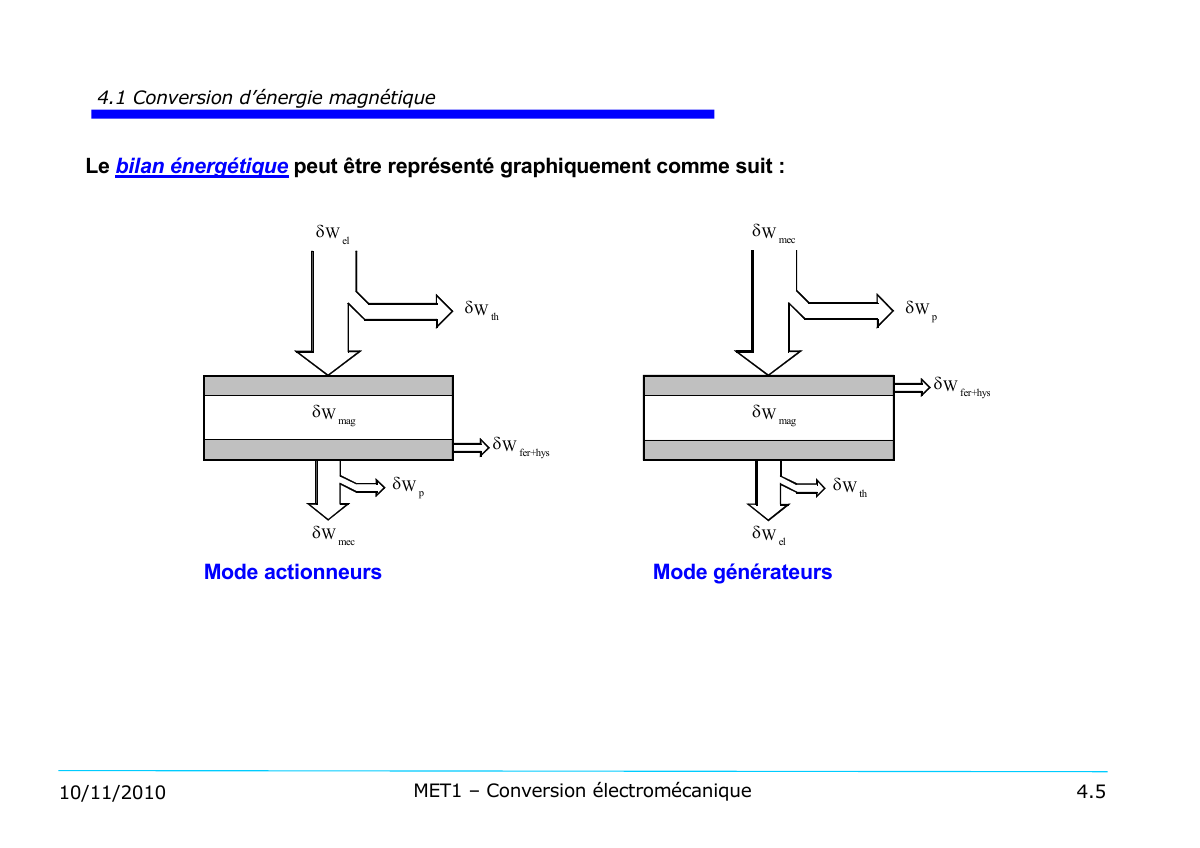
\includegraphics[width=0.78\linewidth]{assets/figures/p4-page-5.png}
\end{center}

\end{metbox}

%====================================================
\begin{metbox}{Énergie et co-énergie magnétiques}

\[
W_{mag}(\Psi,x)=\int_0^\Psi i(\lambda,x)\,d\lambda
\]

\[
W'_{mag}(i,x)=\int_0^i \Psi(\eta,x)\,d\eta
\]

\[
W_{mag}+W'_{mag}=\Psi i
\]

Milieu linéaire :
\[
W_{mag}=W'_{mag}=\frac12Li^2=\frac{\Psi i}{2}
\]

Force/couple par dérivation énergétique :
\[
F_x=-\left.\frac{\partial W_{mag}}{\partial x}\right|_{\Psi}
=\left.\frac{\partial W'_{mag}}{\partial x}\right|_{i}
\]
\[
T=-\left.\frac{\partial W_{mag}}{\partial \alpha}\right|_{\Psi}
=\left.\frac{\partial W'_{mag}}{\partial \alpha}\right|_{i}
\]

\begin{center}
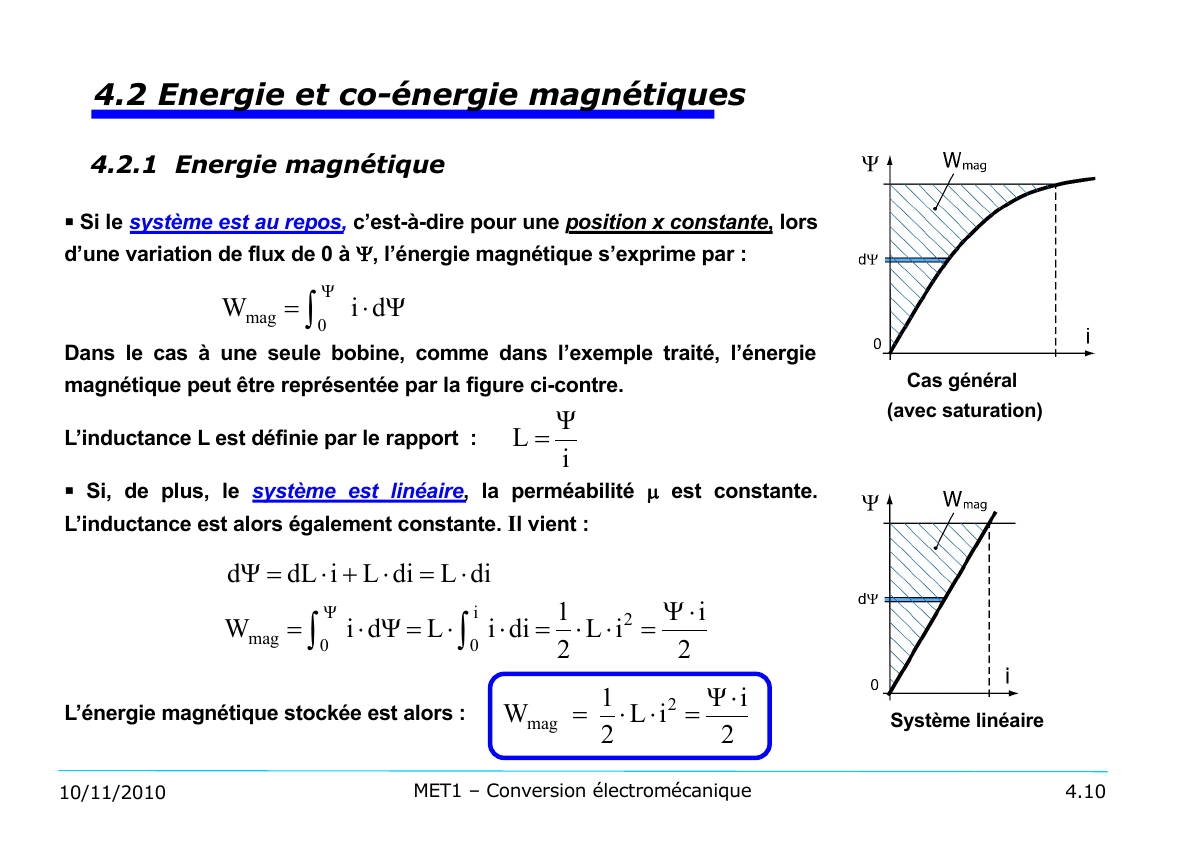
\includegraphics[width=0.78\linewidth]{assets/figures/p4-page-10.png}
\end{center}

\end{metbox}

%====================================================
\begin{metbox}{Systèmes linéaires usuels}

\textbf{1 bobine (réluctant)}
\[
F_x=\frac12\frac{dL}{dx}i^2
\qquad
T=\frac12\frac{dL}{d\alpha}i^2
\]

Avec $\theta=ni$ et $L=n^2\Lambda$ :
\[
F_x=\frac12\frac{d\Lambda}{dx}\theta^2
\qquad
T=\frac12\frac{d\Lambda}{d\alpha}\theta^2
\]

\textbf{2 bobines, 1 ddl rotatif}
\[
T=\frac12\frac{dL_{11}}{d\alpha}i_1^2
+\frac12\frac{dL_{22}}{d\alpha}i_2^2
+\frac{dL_{12}}{d\alpha}i_1i_2
\]

\textbf{Cas général ($k$ circuits, milieu linéaire)}
\[
F_m=\frac12\sum_{j=1}^{k}\sum_{p=1}^{k}
\frac{dL_{jp}}{dx_m}\,i_ji_p
\]
\[
F_m=\frac12\sum_{j=1}^{k}\sum_{p=1}^{k}
\frac{d\Lambda_{jp}}{dx_m}\,\theta_j\theta_p
\]

\textbf{Aimant permanent}
\[
\theta_a=H_cl_a
\qquad
\Phi=\theta_a\Lambda_{eq}
\]
\[
F_x=\frac12\frac{d\Lambda}{dx}\theta_a^2
\]
\[
F_x=\frac{B^2S}{2\mu_0}
\quad (\text{pression magnétique, entrefer})
\]

\end{metbox}

%====================================================
\begin{metbox}{Comportement dynamique}

\textbf{Mouvement}
\[
m\ddot x=F-F_{res}
\qquad
J\ddot\alpha=T-T_{res}
\]

\textbf{Équation électrique}
\[
u_j=R_ji_j+\frac{d\Psi_j}{dt}
\]

Si système non saturé :
\[
\Psi_j=\sum_{p=1}^{k}L_{jp}i_p
\]
\[
u_j=R_ji_j+\sum_{p=1}^{k}L_{jp}\frac{di_p}{dt}
+\sum_{p=1}^{k}i_p\frac{dL_{jp}}{dx}\,v
\]

Tension induite de mouvement :
\[
u_{jm}=\sum_{p=1}^{k}i_p\frac{dL_{jp}}{dx}\,v
=2\frac{F_j}{i_j}v
\]

\textbf{Actionneur électrodynamique (linéaire)}
\[
F=K_Fi,\qquad u_{im}=K_Uv,\qquad K_F=K_U=K
\]
\[
\dot x=v,\quad
\dot v=\frac{1}{m}(K_Fi-C_vv),\quad
\dot i=\frac{1}{L}(u-Ri-K_Uv)
\]

\begin{center}
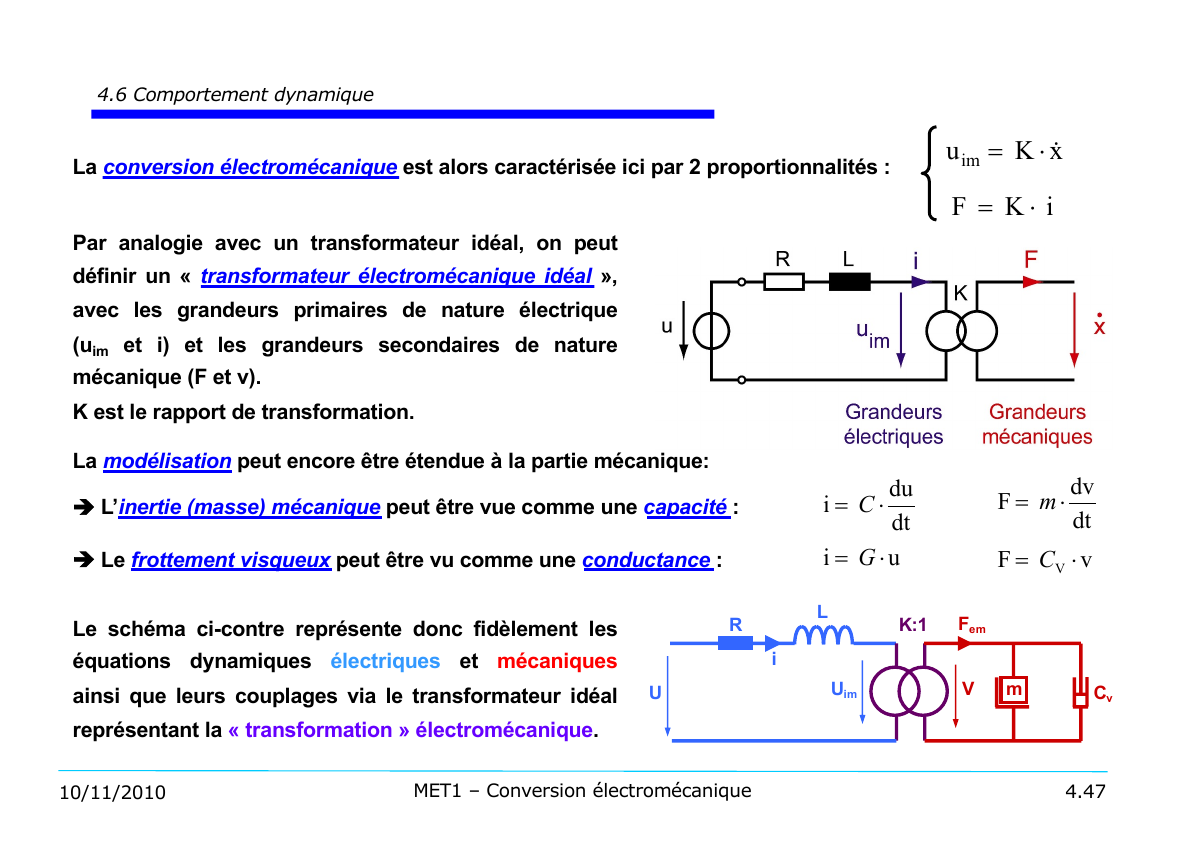
\includegraphics[width=0.78\linewidth]{assets/figures/p4-page-47.png}
\end{center}

\end{metbox}

%====================================================
\begin{metbox}{Rappels utiles pour exercices}

Force d'un électroaimant (sans saturation) :
\[
F_x\propto i^2
\]

Force d'un système électrodynamique (bobine mobile) :
\[
F\propto i
\]

Alimentation AC d'un système réluctant
avec $i(t)=\hat I\sin(\omega t)$ :
\[
F=\frac14\frac{dL}{dx}\hat I^2\left(1-\cos(2\omega t)\right)
\]

Donc :
\[
F=F_{moy}+F_{puls}
\]
avec ondulation de force à la fréquence $2f$.

\end{metbox}

\end{multicols}
}

\end{document}
